% -*- compile-command: "make HOCKING-peak-penalty-slides.pdf" -*-
\documentclass{beamer}
\usepackage{tikz}
\usepackage[all]{xy}
\usepackage{listings}
\usepackage{slashbox}
%\usepackage{booktabs}
\usepackage{amsmath,amssymb}
\usepackage{hyperref}
\usepackage{graphicx}

\DeclareMathOperator*{\argmin}{arg\,min}
\DeclareMathOperator*{\Lik}{Lik}
\DeclareMathOperator*{\Peaks}{Peaks}
\DeclareMathOperator*{\Segments}{Segments}
\DeclareMathOperator*{\argmax}{arg\,max}
\DeclareMathOperator*{\maximize}{maximize}
\DeclareMathOperator*{\minimize}{minimize}
\newcommand{\sign}{\operatorname{sign}}
\newcommand{\RR}{\mathbb R}
\newcommand{\ZZ}{\mathbb Z}
\newcommand{\NN}{\mathbb N}

% Set transparency of non-highlighted sections in the table of
% contents slide.
\setbeamertemplate{section in toc shaded}[default][100]
\AtBeginSection[]
{
  \setbeamercolor{section in toc}{fg=red} 
  \setbeamercolor{section in toc shaded}{fg=black} 
  \begin{frame}
    \tableofcontents[currentsection]
  \end{frame}
}

\begin{document}

\title{PeakSeg: ChIP-seq \textbf{Peak} detection using constrained
  optimal \textbf{Seg}mentation
and supervised penalty learning}  

\author{
  Toby Dylan Hocking\\
  toby.hocking@mail.mcgill.ca\\
  joint work with Guillem Rigaill and Guillaume Bourque}

\date{13 February 2014}

\maketitle

\section{ChIP-seq data and previous work on peak detection}


\begin{frame}
  \frametitle{Chromatin immunoprecipitation sequencing (ChIP-seq)}
  Analysis of DNA-protein interactions.

  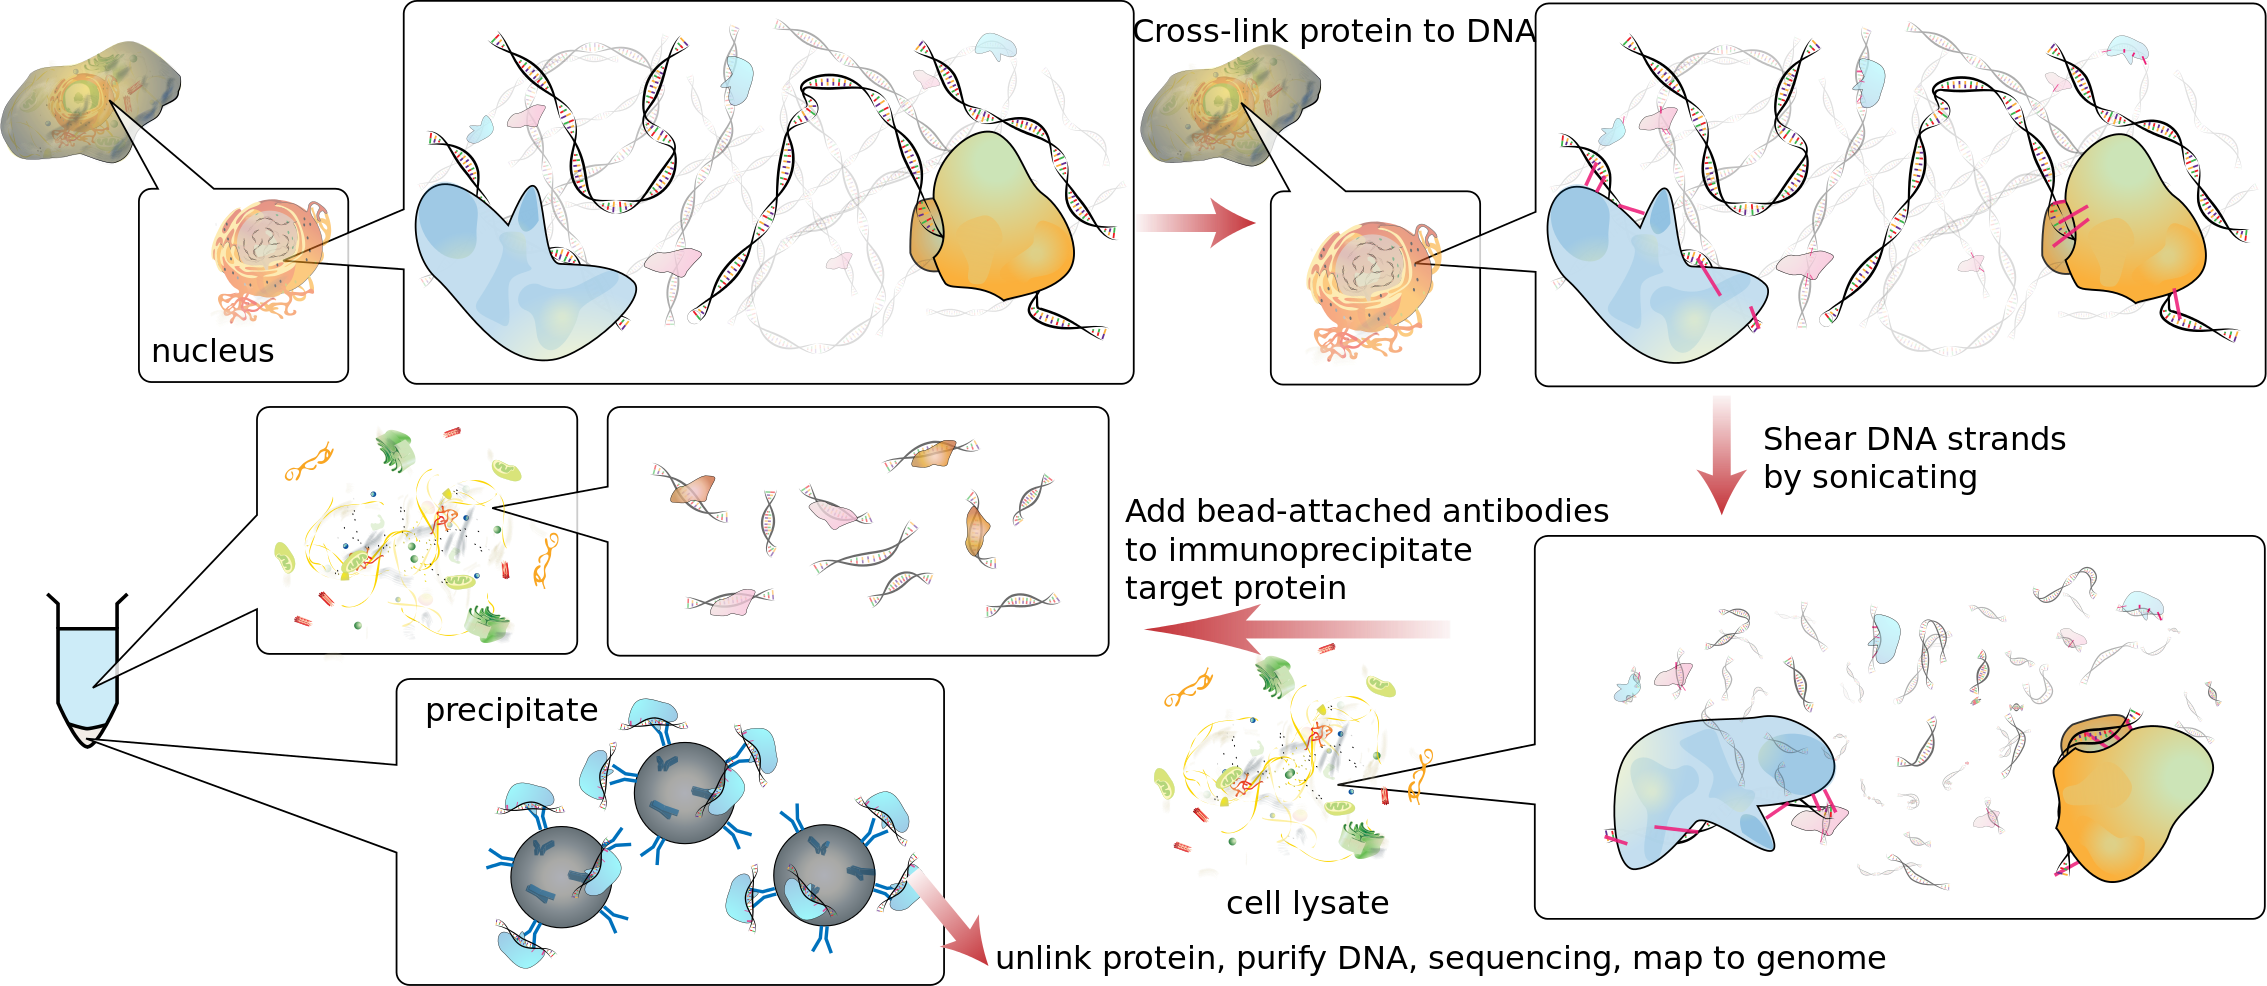
\includegraphics[width=\textwidth]{Chromatin_immunoprecipitation_sequencing_wide.png}

  Source: ``ChIP-sequencing,'' Wikipedia.
\end{frame}

\begin{frame}
  \frametitle{Data downloaded from Epigenomes Portal}
  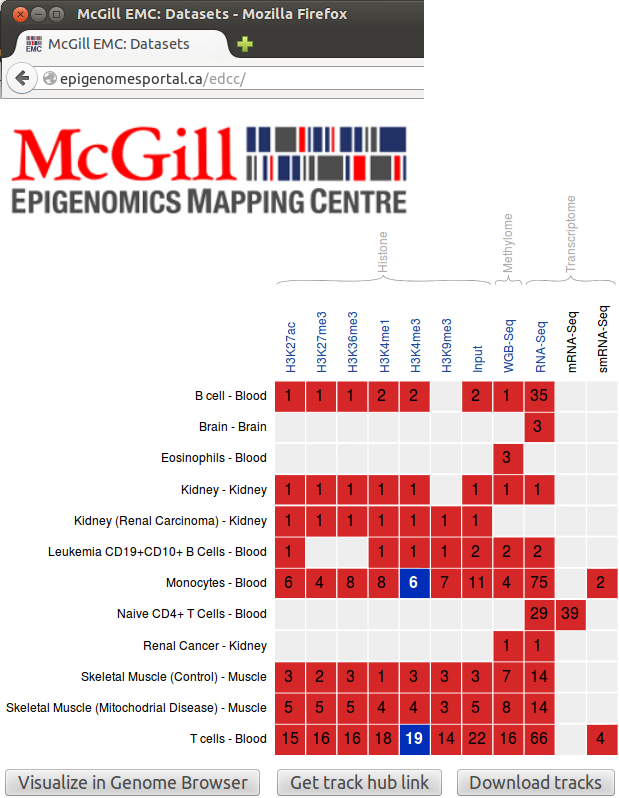
\includegraphics[width=2.5in]{screenshot-samples}
\end{frame}

\begin{frame}
  \frametitle{Problem: find peaks in each of several samples}
  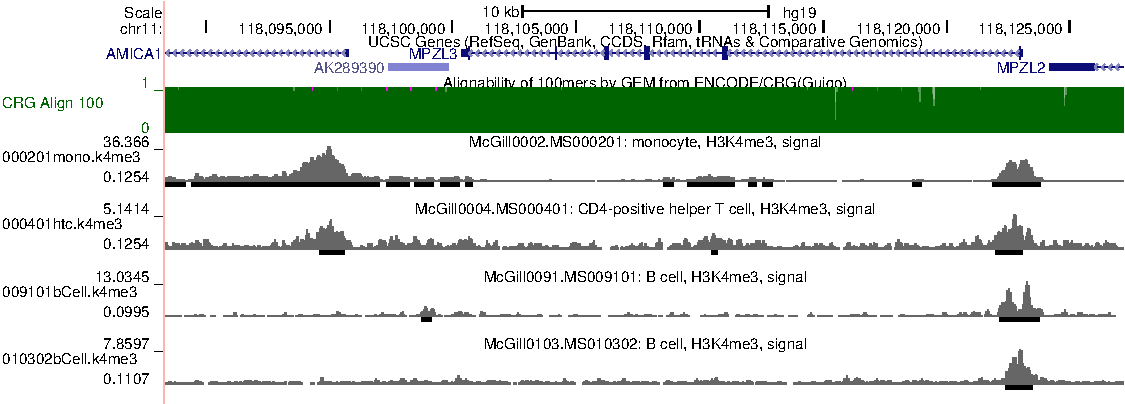
\includegraphics[width=\textwidth]{screenshot-ucsc-edited}
\end{frame}

\begin{frame}
  \frametitle{Existing peak detection algorithms}
  \begin{itemize}
  \item Model-based analysis of ChIP-Seq (MACS), Zhang et al, 2008.
  \item SICER, Zang et al, 2009.
  \item HOMER findPeaks, Heinz et al, 2010.
  \item RSEG, Song and Smith, 2011.
  \item Histone modifications in cancer (HMCan), Ashoor et al, 2013.
  \item ... dozens of others.
  \end{itemize}
  Two big questions: how to choose the best...
  \begin{itemize}
  \item ...algorithm?
  \item ...parameters?
  \end{itemize}
\end{frame}

\begin{frame}[fragile]
  \frametitle{How to choose model parameters?}
\scriptsize
19 parameters for Model-based analysis of ChIP-Seq (MACS), Zhang et al, 2008.
\begin{verbatim}
  [-g GSIZE]
  [-s TSIZE] [--bw BW] [-m MFOLD MFOLD] [--fix-bimodal]
  [--nomodel] [--extsize EXTSIZE | --shiftsize SHIFTSIZE]
  [-q QVALUE | -p PVALUE | -F FOLDENRICHMENT] [--to-large]
  [--down-sample] [--seed SEED] [--nolambda]
  [--slocal SMALLLOCAL] [--llocal LARGELOCAL]
  [--shift-control] [--half-ext] [--broad]
  [--broad-cutoff BROADCUTOFF] [--call-summits]
\end{verbatim}
10 parameters for Histone modifications in cancer (HMCan),
Ashoor et al, 2013.
\begin{verbatim}
minLength 145
medLength 150
maxLength 155
smallBinLength 50
largeBinLength 100000
pvalueThreshold 0.01
mergeDistance 200
iterationThreshold 5
finalThreshold 0
maxIter 20
\end{verbatim}
\end{frame}

\begin{frame}
  \frametitle{Previous work in computer vision: look and add labels
    to...}
  \begin{tabular}{ccc}
    Photos & Cell images & Copy number profiles \\
    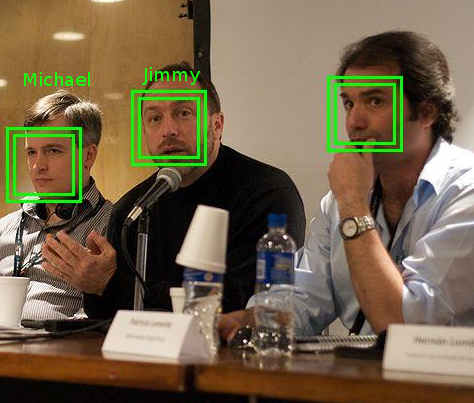
\includegraphics[width=1.3in]{faces} &
    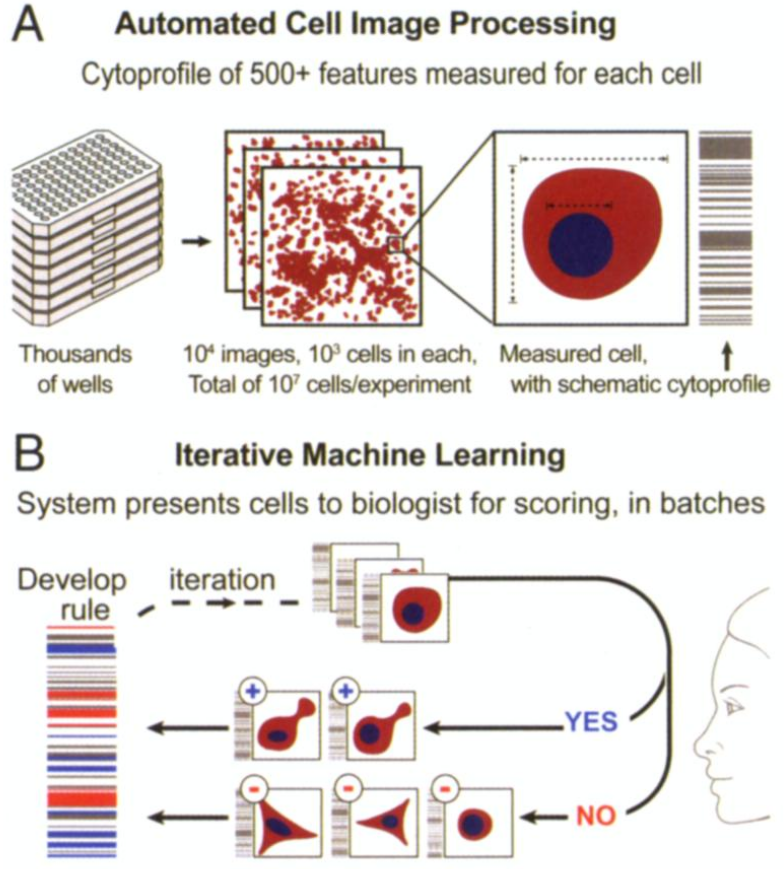
\includegraphics[width=1.3in]{cellprofiler} &
    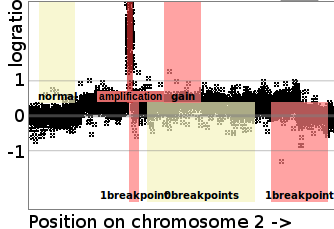
\includegraphics[width=1.5in]{regions-axes}\\
    Labels: names & phenotypes & alterations \\ \\
    CVPR 2013 & CellProfiler & SegAnnDB \\
    246 papers & 873 citations & H, \emph{et. al.} 2014. \\
     &
  \end{tabular}
  Sources: \url{http://en.wikipedia.org/wiki/Face_detection}\\
  Jones et al PNAS 2009. Scoring diverse cellular morphologies in
  image-based screens with iterative feedback and machine learning.
\end{frame}

% \begin{frame}
%   \frametitle{Peak H3K4me3 profiles with manually annotated regions}
%   \includegraphics[width=\textwidth]{figure-macs-default-4samples-just-regions}

%   Determined by visual inspection on
%   \href{http://ucscbrowser.genap.ca/cgi-bin/hgTracks?db=hg19\&position=chr11:118080000-118130000}{ucscbrowser.genap.ca}
% \end{frame}

% \begin{frame}
%   \frametitle{Peak H3K4me3 profiles, macs default model}
%   \includegraphics[width=\textwidth]{figure-macs-default-4samples-with-peaks}

%   How many errors?
% \end{frame}

% \begin{frame}
%   \frametitle{Peak H3K4me3 profiles, macs default model}
%   \includegraphics[width=\textwidth]{figure-macs-default-4samples}

%   3 false positives, 2 false negatives.
% \end{frame}

% \begin{frame}
%   \frametitle{Peak H3K4me3 profiles, macs trained model}
%   \includegraphics[width=\textwidth]{figure-macs-4samples}

%   1 false positive, 3 false negatives.
% \end{frame}

% \begin{frame}
%   \frametitle{Broad H3K36me3 profiles, HMCan.broad default model}
%   \includegraphics[width=\textwidth]{figure-H3K36me3-sub-hmcan-broad-2}

%   13 false positives, 1 false negative.
% \end{frame}

% \begin{frame}
%   \frametitle{Broad H3K36me3 data, HMCan.broad trained model}
%   \includegraphics[width=\textwidth]{figure-H3K36me3-sub-hmcan-broad-1}

%   0 false positives, 2 false negatives.
% \end{frame}

\begin{frame}
  \frametitle{Comparison on annotated McGill benchmark data set}
  Hocking et al, 2014, arXiv:1409.6209.\\
  \begin{itemize}
  \item Manually annotate regions with or without peaks.\\
    \url{http://cbio.ensmp.fr/~thocking/chip-seq-chunk-db/}
  \item Tune 1 parameter that affects the number of peaks.
  \item Choose the parameter that minimizes the annotation error.
  \end{itemize}
  Results:
  \begin{itemize}
  \item MACS best for H3K4me3 (sharp peak pattern),
  \item HMCan.broad best for H3K36me3 (broad peak pattern).
  \item 10--20\% test error rates.
  \item Same results across 4 annotators (PhD students, postdocs).
  \end{itemize}
\end{frame}

\begin{frame}
  \frametitle{Two annotators provide consistent labels, but different
    precision}
  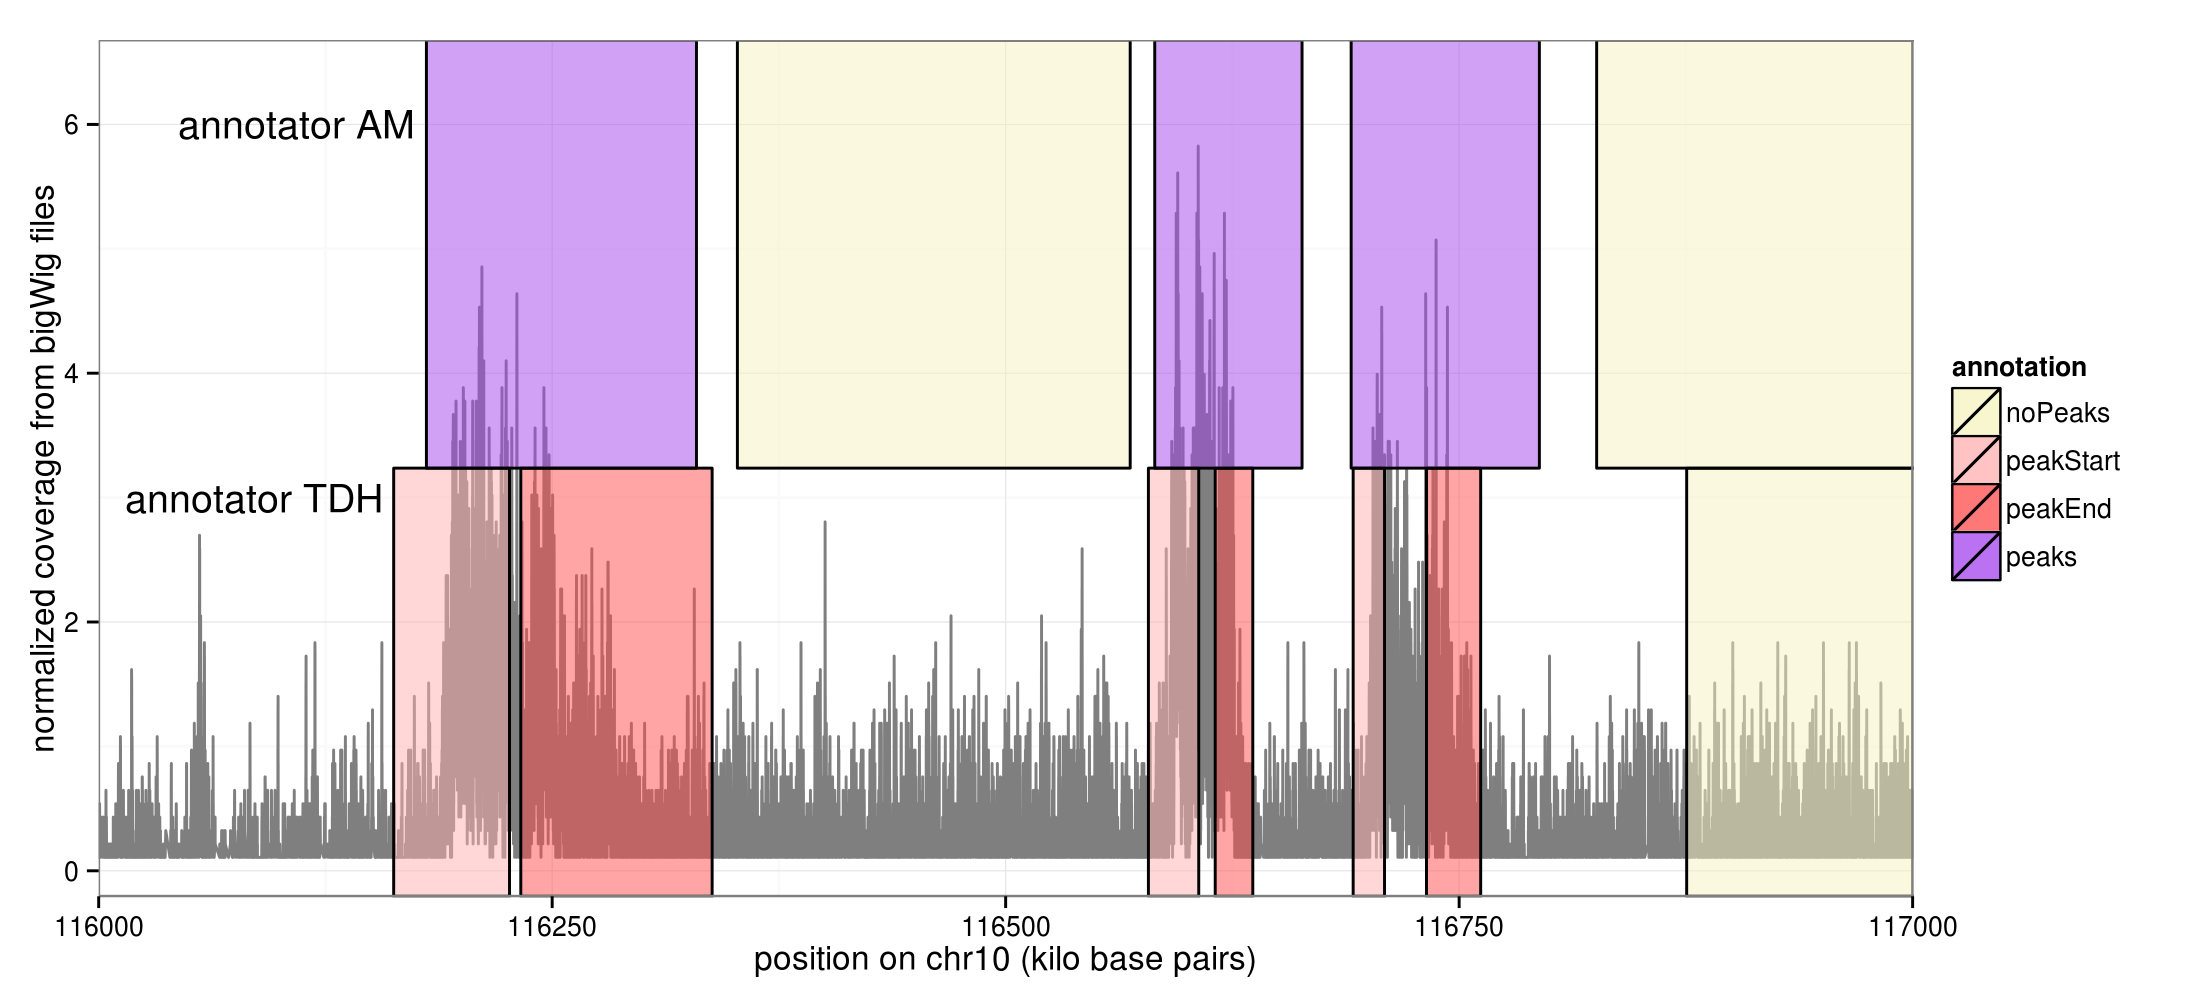
\includegraphics[width=1.1\textwidth]{figure-several-annotators}

  \begin{itemize}
  \item TDH peakStart/peakEnd more precise than AM peaks.
  \item AM noPeaks more precise than TDH no label.
  \end{itemize}
\end{frame}

\begin{frame}
  \frametitle{Can we do better than unsupervised peak detectors? Yes!}
  We propose \textbf{PeakSeg}, a new model with efficient algorithms
  for supervised peak detection.
  \begin{itemize}
  \item Input: \alert<1>{several ChIP-seq profiles},
    \alert<2>{manually annotated regions}.
  \item New methods for peak detection: 
    \begin{itemize}
    \item \alert<1>{Constrained optimal segmentation}.
    \item Efficient \alert<2>{supervised learning using manually annotated
      regions}.
    \end{itemize}
  \item Output: predicted peaks for each profile.
  %\item and consistent peak boundaries across samples.
  \end{itemize}
  State-of-the-art peak detection accuracy (on both sharp H3K4me3 and
  broad H3K36me3 profiles).
\end{frame}

\section{Methods: constrained optimal segmentation and 
  supervised penalty learning}

\input{figure-dp-first}

\input{figure-dp-short}

\input{figure-dp}

% \begin{frame}
%   \frametitle{Previous work: maximum likelihood segmentation}
%   \begin{itemize}
%   \item   Let $\mathbf y = 
% \left[
%   \begin{array}{ccc}
%     y_1 & \cdots & y_d
%   \end{array}
% \right]
% \in\ZZ_+^d$ be the aligned read counts for one sample
%   and one chromosome.
% \item For example the biggest chromosome in hg19 (chr1) has
%   $d=249,250,621$ bases.
% \item For each number of segments $s\in\{1, \dots,
%   s_{\text{max}}\}$, we want:
%   \end{itemize}
%   \begin{equation*}
%     \label{argmax:M}
%     \begin{aligned}
%       \mathbf{\hat m}^s(\mathbf y)  =\ 
%       &\argmax_{\mathbf m\in\RR^{d}} && \sum_{j=1}^d
%       \log\Lik(y_{j}, m_{j}) \\
%       \\
%       &\text{such that} && \Segments(\mathbf m)=s.
%     \end{aligned}
%   \end{equation*}
%   \begin{itemize}
%   \item Only one free parameter $s_{\text{max}}$, the maximum number
%     of segments per chromosome.
%   \item Pruned Dynamic Programming (Rigaill arXiv:1004.0887) returns
%     $\mathbf{\hat m}^1(\mathbf y), \dots, \mathbf{\hat
%       m}^{s_{\text{max}}}(\mathbf y)$ in $O(s_{\text{max}} d\log d)$
%     time.
%   \end{itemize}
% \end{frame}

% \begin{frame}
%   \frametitle{Maximum likelihood segmentation models}
%   \includegraphics[width=\textwidth]{figure-Segmentor-nopeaks-notext}

%   Poisson likelihood, implemented in Segmentor3IsBack R package
%   (Cleynen et al. 2014).

%   %50,000 base pairs and 3,463 weighted data segments.
% \end{frame}

% \begin{frame}
%   \frametitle{PeakSeg:  constrained maximum likelihood
%     segmentation}
%   \begin{itemize}
% \item For each number of peaks $p\in\{0, 1, \dots,
%   p_{\text{max}}\}$, we want:
%   \end{itemize}
%   \begin{equation*}
%     \label{argmax:M}
%     \begin{aligned}
%       \mathbf{\tilde m}^p(\mathbf y)  =\ 
%       &\argmax_{\mathbf m\in\RR^{d}} && \sum_{j=1}^d
%       \log\Lik(y_{j}, m_{j}) \\
%       \\
%       &\text{such that} && \Peaks(\mathbf m)=p.
%     \end{aligned}
%   \end{equation*}
%   \begin{itemize}
%   \item Only one free parameter $p_{\text{max}}$, the maximum number
%     of peaks per chromosome.
%   \item We propose Constrained 
%     %Pruned 
%     Dynamic Programming, which
%     returns $\mathbf{\tilde m}^0(\mathbf y), \dots, \mathbf{\tilde
%       m}^{p_{\text{max}}}(\mathbf y)$ 
%     %in $O(p_{\text{max}} d\log d)$ time.
%     in $O(p_{\text{max}} d^2)$ time.
%   \end{itemize}
% \end{frame}

% \begin{frame}
%   \frametitle{Part of one H3K4me3 ChIP-seq profile}
%   \includegraphics[width=\textwidth]{figure-PeakSeg-neither}

%   Noisy ChIP-seq data only.
% \end{frame}

% \begin{frame}
%   \frametitle{PeakSeg models from 0 to 3 peaks}
%   \includegraphics[width=\textwidth]{figure-PeakSeg-seg}

%   Data and segmentation.
% \end{frame}

% \begin{frame}
%   \frametitle{PeakSeg models from 0 to 3 peaks}
%   \includegraphics[width=\textwidth]{figure-PeakSeg}

%   Data, segmentation, and peaks.
% \end{frame}

% \begin{frame}
%   \frametitle{PeakSeg models from 0 to 3 peaks}
%   \includegraphics[width=\textwidth]{figure-PeakSeg-peaks}

%   Data and peaks.
% \end{frame}

% \begin{frame}
%   \frametitle{PeakSeg models from 0 to 3 peaks}
%   \includegraphics[width=\textwidth]{figure-PeakSeg-regions}

%   Peaks and annotated regions.
% \end{frame}

% \begin{frame}
%   \frametitle{PeakSeg on several samples}
%   \begin{itemize}
%   \item Let there be $n$ samples of aligned read counts
%   $\mathbf y_1\in\ZZ_+^d, \dots, \mathbf y_n\in\ZZ_+^d$
%   on a chromosome with $d$ base pairs.
% \item For each sample, compute a sequence of models with
%   $p\in\{0,\dots, p_{\text{max}}\}$ peaks.
%   \item Sample 1: $\mathbf {\tilde m}^0(\mathbf y_1), 
%     \dots, 
%     \mathbf{\tilde m}^{p_{\text{max}}}(\mathbf y_1)$,
%   \\ $\vdots$
%   \item Sample $n$: $\mathbf {\tilde m}^0(\mathbf y_n), 
%     \dots, 
%     \mathbf{\tilde m}^{p_{\text{max}}}(\mathbf y_n)$.
%   \item Parallelizable on samples and chromosomes.
%   \end{itemize}
% \end{frame}

% \begin{frame}
%   \frametitle{H3K4me3 data, PeakSeg models with 1 peak}
%   \includegraphics[width=\textwidth]{figure-PeakSeg1-4samples}
% \end{frame}

% \begin{frame}
%   \frametitle{H3K4me3 data, PeakSeg models with 2 peaks}
%   \includegraphics[width=\textwidth]{figure-PeakSeg2-4samples}
% \end{frame}

% \begin{frame}
%   \frametitle{H3K4me3 data, PeakSeg models with 3 peaks}
%   \includegraphics[width=\textwidth]{figure-PeakSeg3-4samples}
% \end{frame}

% \begin{frame}
%   \frametitle{H3K36me3 data, PeakSeg model with 1 peak}
%   \includegraphics[width=\textwidth]{figure-H3K36me3-sub-PeakSeg-1}
% \end{frame}

% \begin{frame}
%   \frametitle{H3K36me3 data, PeakSeg model with 2 peaks}
%   \includegraphics[width=\textwidth]{figure-H3K36me3-sub-PeakSeg-2}
% \end{frame}

% \begin{frame}
%   \frametitle{H3K36me3 data, PeakSeg model with 3 peaks}
%   \includegraphics[width=\textwidth]{figure-H3K36me3-sub-PeakSeg-3}
% \end{frame}

\begin{frame}
  \frametitle{Summary of unsupervised PeakSeg algorithm}
  Parallelizable on samples/chromosomes:
  \begin{itemize}
  \item Inputs: a ChIP-seq coverage profile $\mathbf y\in\ZZ_+^d$ on a
    chromosome with $d$ base pairs, maximum number of peaks
    $p_{\text{max}}$.
  \item Proposed method: constrained 
    %pruned 
    dynamic programming
    algorithm,
    %$O(p_{\text{max}} d \log d)$ time complexity.
    $O(p_{\text{max}} d^2)$ time complexity.
  \item Outputs: constrained maximum likelihood segmentations
    $\mathbf{\tilde m}^0(\mathbf y), 
    \dots, 
    \mathbf{\tilde m}^{p_{\text{max}}}(\mathbf y)$ 
    (peaks are 2nd, 4th, ... segments).
  \end{itemize}
  How to choose the optimal number of peaks?\\
  Manually annotated regions + supervised learning (next slide).
\end{frame}

\begin{frame}
  \frametitle{Previous work on breakpoint detection}
  G Rigaill, TD Hocking, \emph{et al.} Learning Sparse Penalties for Change
  Point Detection using Max Margin Interval Regression, ICML 2013.
  \begin{itemize}
  \item Supervised algorithm for detecting change points in piecewise
    constant DNA copy number profiles.
  \item Inputs: genomic profile $\mathbf y$, \\
    profile features $\mathbf x$, \\
    manually annotated regions $R$ (change point locations).
  \item Method: compute maximum likelihood segmentations $\mathbf{\hat
      m}^1(\mathbf y), \dots, \mathbf{\hat m}^{s_{\text{max}}}(\mathbf
    y)$, learn a penalty function $f(\mathbf x) \Rightarrow \hat s$
    that minimizes the number of incorrect regions $R$.
    \item Output: the segmentation with minimum predicted error
      $\mathbf{\hat m}^{\hat s}(\mathbf y)$.
  \end{itemize}
  We can use the same method for peak detection!
\end{frame}

\section{Results on the McGill benchmark data set, conclusions}

\begin{frame}
  \frametitle{Benchmark: 7 annotated region data sets}
  \url{http://cbio.ensmp.fr/~thocking/chip-seq-chunk-db/}
  \begin{itemize}
  \item 4 annotators (AM, TDH, PGP, XJ).
  \item 8 cell types.
  \item 37 annotated H3K4me3 profiles (sharp peaks).
  \item 29 annotated H3K36me3 profiles (broadly enriched domains).
  \item 12,826 annotated regions in total.
  \end{itemize}
  Used the DP algorithm on a subset of the data.
  \begin{itemize}
  \item Compute 10 PeakSeg models $\mathbf{\tilde m}^1(\mathbf
    y),\mathbf{\tilde m}^3(\mathbf y), \dots, \mathbf{\tilde
      m}^{19}(\mathbf y)$.
  \item For the biggest window, DP took 3 hours.\\
    ($d=88,509$ data points, 3.5  megabases)
  \item macs takes about 90 minutes for one whole genome.
  \end{itemize}
\end{frame}

\begin{frame}
  \frametitle{Penalty functions learned in this paper}

Predicted number of segments for profile $i\in\{1, \dots, n\}$:

\begin{equation*}
  \hat s_i = 
  \argmin_{s\in\{1,3,\dots, s_{\text{max}}=19\}}
  \overbrace{\rho\left[
    \mathbf{\tilde m}^s(\mathbf y_i),
    \mathbf y_i
  \right]}^{\text{loss}}
  + 
  \overbrace{
    \alert<3>{\lambda_i}
    \alert<2>{h(s, d_i)}
  }^{\text{penalty}},
\end{equation*}

  Names: (model complexity).(number of parameters learned):

  \begin{center}
  \begin{tabular}{ll}
    \textbf{name} & \textbf{model complexity} \alert<2>{$h(s, d_i)$} \\
    \hline
    AIC/BIC.* & \alert<2>{$s$}\\
    oracle.* & \alert<2>{$s\left(1 + 4\sqrt{1.1 + \log(d_i/s)}\right)^2$}
  \end{tabular}
\end{center}

  \begin{center}
  \begin{tabular}{lllll}
    \textbf{name} & \textbf{smoothing} \alert<3>{$\lambda_i$} & 
    \textbf{parameters} & \textbf{learning algorithm} \\
    \hline
    *.0 & AIC=\alert<3>{2}, BIC=\alert<3>{$\log d_i$} & none & unsupervised \\
    *.1 & 
    \alert<3>{$\beta$} & 
    $\beta\in\RR_+$ & grid search \\
    *.3 & 
    \alert<3>{$e^\beta d_i^{w_1} (\max \mathbf y_i)^{w_{2}}$} & 
    $\beta, w_1, w_{2}\in\RR$ & interval regression \\
    *.41 & 
    \alert<3>{$\exp(\beta + \mathbf w^\intercal \mathbf x_i)$} & 
    $\beta\in\RR, \mathbf w\in\RR^{40}$ & 
    interval regression \\
  \end{tabular}
\end{center}

($d_i$ = number of data for profile $i$)

\end{frame}

\begin{frame}
  \frametitle{Unsupervised constrained optimization algorithm works
    for both H3K36me3 and H3K4me3 data types}

  ...except in the H3K4me3\_XJ\_immune data set.

  \includegraphics[width=\textwidth]{figure-dp-peaks-regression-dots-unsupervised}
  
  Six train/test splits (open circles) and mean (shaded circle).
\end{frame}

\begin{frame}
  \frametitle{Training 1 parameter with grid search reduces test error}

  ...except for macs, good defaults for 3/4 H3K4me3 data sets.

  \includegraphics[width=\textwidth]{figure-dp-peaks-regression-dots-grid}

  Six train/test splits (open circles) and mean (shaded circle).
\end{frame}

\begin{frame}
  \frametitle{Training several parameters with interval regression 
    further reduces test error}

  ...except when there are few train data (H3K36me3\_TDH).

  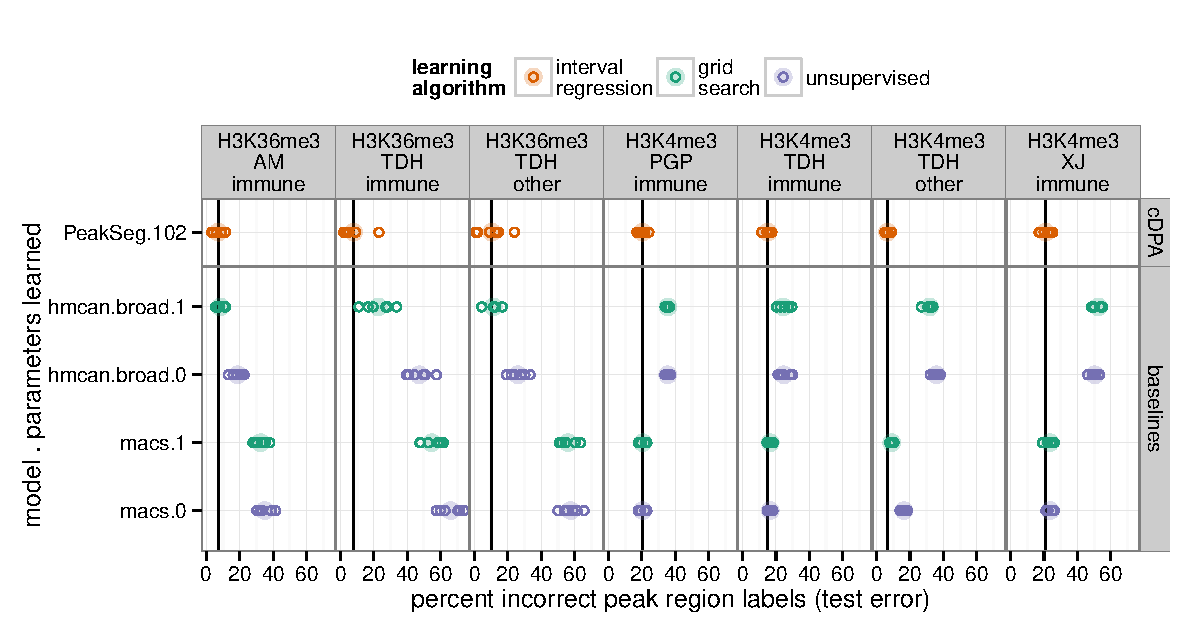
\includegraphics[width=\textwidth]{figure-dp-peaks-regression-dots}

  Six train/test splits (open circles) and mean (shaded circle).
\end{frame}

\begin{frame}
  \frametitle{Conclusions and future work}
  PeakSeg: \textbf{Peak} detection via constrained optimal
  \textbf{Seg}mentation.
  \begin{itemize}
  \item First peak detector with efficient multi-parameter supervised
    learning algorithm.
  \item State-of-the-art peak detection for both H3K4me3 and H3K36me3
    profiles.
  \end{itemize}
  Future work:
  \begin{itemize}
  \item Constrained version of Pruned Dynamic Programming (Rigaill
    arXiv:1004.0887) to compute PeakSeg in $O(d\log d)$ time.
  \item Apply to whole genome (not just annotated windows).
  \item Better test error using other features $\mathbf x$?
  \item Detecting the same peaks across several profiles?
  \end{itemize}
\end{frame}

\section{Google Summer of Code}

\begin{frame}
  \frametitle{Google Summer of Code (GSOC)}
Student gets \$5000 for writing open source code for
    3 months.
    \begin{description}
    \item[Feb] \textbf{Admins} for open source organizations
      e.g. R, Bioconductor apply to Google.
    \item[Mar] \textbf{Mentors} suggest projects for each org.\\
      \textbf{Students} submit project proposals to Google.\\
      Google gives funding for $n$ students to an org.
    \item[April] The top $n$ students get \$500 and begin coding.
    \item[July] Midterm evaluation, pass = \$2250.
    \item[Aug] Final evaluation, pass = \$2250.
    \item[November] Orgs get \$500/student mentored.
    \end{description}

  I have participated as an \textbf{admin} and \textbf{mentor} for the
  R project.
\end{frame}

\begin{frame}
  \frametitle{What makes a good GSOC project?}
  Coding projects should:
  \begin{itemize}
  \item Result in free/open-source software.
  \item Be 3 months of full time work for a student.
  \item Include writing documentation and tests.
  \item Not include original research.
  \end{itemize}
  Examples: 
  \begin{itemize}
  \item Louis/Mathieu can be \textbf{admins} for MUGQIC org.
  \item Warren/Stephan can be \textbf{mentors} for a project to write
    a new R package for methylation analysis.
  \item Robert/Dan can be \textbf{mentors} for a project to implement
    new features in Gemini.
  \item Any undergrad/master/PhD candidates (at McGill or not)
    can be \textbf{students}.
  \end{itemize}
  
\end{frame}

\begin{frame}
  \frametitle{Thanks for your attention!}
  Write me at \alert{\texttt{toby.hocking@mail.mcgill.ca}} to collaborate!

  \vskip 1cm

  Source code for slides online!\\
  \small
  \url{https://github.com/tdhock/PeakSeg-paper/HOCKING-PeakSeg-slides.tex}
  \vskip 1cm

  Supplementary slides appear after this one.

\end{frame}

\begin{frame}
  \frametitle{Definition of Peaks model complexity function}
  $S_1(\mathbf m)=0$, direction of change before base $j\in\{2, \dots, d\}$:
  \begin{equation*}
    \label{eq:S_j}
    S_j(\mathbf m) = \sign( m_{j} - m_{j-1} ),
  \end{equation*}

  Number of peaks at base $j\in\{1, \dots, d\}$:
  \begin{equation*}
    \label{eq:P_j}
    P_j(\mathbf m) = \sum_{k=1}^j S_k(\mathbf m).
  \end{equation*}

  Peaks must be larger than background:
  \begin{equation*}
    \label{eq:C_j}
    C_j(\mathbf m) =
    \begin{cases}
      \infty & \text{ if } P_j(\mathbf m) < 0,\\
      0 & \text{ otherwise.}
    \end{cases}
  \end{equation*}
  
  Finally,
  \begin{equation*}
    \label{eq:Peaks}
    \Peaks(\mathbf m) =
    \sum_{j=1}^d 
    C_j(\mathbf m) +
    S_j(\mathbf m)_+.
  \end{equation*}
  
\end{frame}

% \begin{frame}
%   \frametitle{Same peaks detected using 3 different representations}
%   \includegraphics[width=0.9\textwidth]{figure-PeakSeg-first-last}
% \end{frame}

\begin{frame}
  \frametitle{Step 1: compute annotation error functions}
  \begin{itemize}
  \item Inputs: for $i\in\{1, \dots, n\}$ samples, genomic profiles
    $\mathbf y_i$, annotated regions $R_i$.
    \begin{equation*}
      \begin{array}{cccc}
        & \text{0 peaks} & \cdots & \text{$p_{\text{max}}$ peaks}\\
        \hline
        \text{segmentations} &
        \mathbf{\tilde m}^0(\mathbf y_i) & 
        \cdots & 
        \mathbf{\tilde m}^{p_{\text{max}}}(\mathbf y_i)\\
        \text{annotation error} & 
        e_i(0) &
        \cdots & 
        e_i(p_{\text{max}})\\
      \end{array}
    \end{equation*}
  \item R package \url{https://github.com/tdhock/PeakError/} computes
    the \textbf{annotation error}
    $e_i:\{0,\dots,p_{\text{max}}\}\rightarrow \ZZ_+$.
  \item   TD Hocking \emph{et al.} Visual annotations and a supervised
    learning approach for evaluating and calibrating ChIP-seq peak detectors
    (arXiv:1409.6209).
  \end{itemize}
\end{frame}

\begin{frame}
  \frametitle{Step 2: compute model selection functions}
  For each sample/chromosome $i\in\{1, \dots, n\}$, for $\lambda\in\RR_+$,
  \begin{itemize}
  \item   The \textbf{optimal number of peaks} function is
  \begin{equation*}
    p_i^*(\lambda) = \argmin_{p\in\{1,\dots, p_{\text{max}}\}}
      \alpha_i^p + \lambda p,
  \end{equation*}
  where  $\alpha_i^p$ is the Poisson loss of the model with $p$ peaks.
  % \begin{equation*}
  %   \label{eq:loss}
  %   L_i^p = \sum_{j=1}^d \tilde m^p_{ij} - y_{ij} \log \tilde m^p_{ij}.
  % \end{equation*}
  \item The \textbf{penalized annotation error} function is
  \begin{equation*}
    E_i(\lambda) = e_i\left[ p_i^*(\lambda) \right],
  \end{equation*}
  where $e_i(p)$ is the number of incorrect annotations for the model
  with $p$ peaks.
  \end{itemize}
  \textbf{Peaks $p_i^*$ and error $E_i$ are non-convex, piecewise
    constant functions that can be computed exactly.}
\end{frame}
 
\begin{frame}
  \frametitle{Step 3: learn a penalty function via interval regression}
  \begin{itemize}
  \item Compute the target interval $(\underline L_i, \overline
    L_i)$.
  \item $\log \lambda_i\in(\underline L_i, \overline L_i) \Rightarrow$
   optimal peak detection.
  \item Compute simple features $\mathbf x_i\in\RR^m$, e.g. chromosome size,
    read counts, signal scale $\log \max \mathbf y_i $.
  \item Learn an optimal affine $f(\mathbf x_i) =
    \beta + \mathbf w^\intercal \mathbf x_i = \log \lambda_i $.
    % \begin{equation*}
    %   \minimize_{\beta\in\RR, \mathbf w\in\RR^m} \sum_{i=1}^n \ell\left[
    %     (\underline L_i, \overline L_i),
    %     \beta + \mathbf w^\intercal \mathbf x_i 
    %   \right]
    %   + ||w||_1.
    % \end{equation*}
  \item Equivalent to learning a penalty $\lambda_i = \exp
    f(\mathbf x_i)$:
    \begin{eqnarray*}
  p_i^*[\exp f(\mathbf x_i)] 
&=& \argmin_p  \alpha_i^p +  p \exp f(\mathbf x_i) \\
&=& \argmin_p \alpha_i^p + p (\max \mathbf y_i)^w e^\beta.
\end{eqnarray*}
  \item Convex optimization problem, global optimum, variable
    selection (G Rigaill, TD Hocking, \emph{et al.} ICML 2013).
  \end{itemize}
\end{frame}

\begin{frame}
  \frametitle{Summary of supervised PeakSeg 
     algorithm}
  \begin{itemize}
  \item Fix the maximum number of peaks $p_{\text{max}} = 10,000$.
  \item For each sample/chromosome $i\in\{1,\dots, n\}$,
    \begin{itemize}
    \item \textbf{Unsupervised PeakSeg}: compute constrained maximum likelihood
      segmentations $\mathbf{\tilde m}^0(\mathbf y_i), \dots,
      \mathbf{\tilde m}^{p_{\text{max}}}(\mathbf y_i)$.
    \item Step 1: use annotated region labels to compute the
      annotation error $e_i(0), \dots, e_i(p_{\text{max}})$.
    \item Step 2: compute peaks $p_i^*(\lambda)$, error
      $E_i(\lambda)$, and target interval $(\underline L_i, \overline
      L_i)$.
    \end{itemize}
  \item  Step 3:  learn a  penalty $\lambda_i  = \exp  f(\mathbf x_i)$
    using features $\mathbf x_i$ such as $\log \max(\mathbf y_i)$.
  \item Given an unlabeled chromosome $(\mathbf x, \mathbf y)$, we predict
    $\mathbf{ \tilde m}^{p^*\left[
        \exp f(\mathbf x)
      \right]}(\mathbf y)$.
  %\item Optional post-processing: mean of overlapping peaks.
  \end{itemize}
\end{frame}

\end{document}
